\section{Tool Support and Future Work}
\label{sec:toolsupport}
\subsection{Assurance Case Modelling Environment - ACME}
With all its power in model-based system assurance, there is one drawback for SACM at the moment, which is the lack of concrete syntax, i.e. graphical representations of SACM\footnote{Graphical syntax for SACM is being developed by us}. 
Without graphical representations, it is typically difficult for engineers to construct SACM. 
Hence, in order to exploit the benefits provided by SACM whilst provide support for existing assurance case approaches, we started developing a tool (Assurance Case Modelling Environment, ACME\footnote{Available upon request.}) based on SACM and the GSN metamodel we discussed in Section~\ref{sec:mapping}. 

\begin{figure}
	\centering
	\begin{minipage}[b]{0.49\textwidth}
		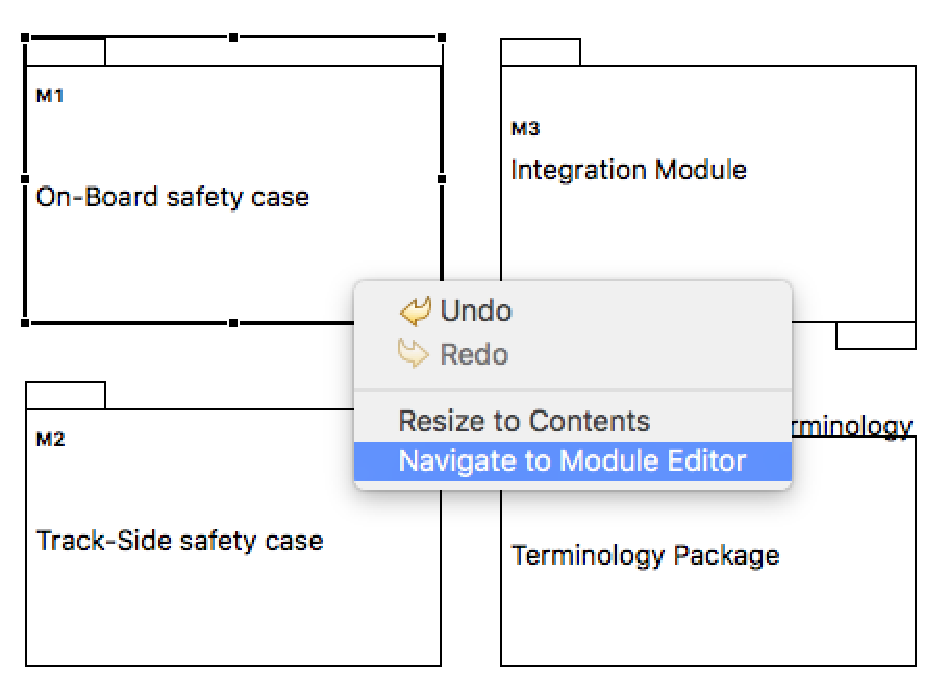
\includegraphics[width=1\linewidth]{ac_view.pdf}
		\caption{The Assurance Case Package View of ACME.}
		\label{fig:ac_view}
	\end{minipage}
	\hfill
	\begin{minipage}[b]{0.49\textwidth}
		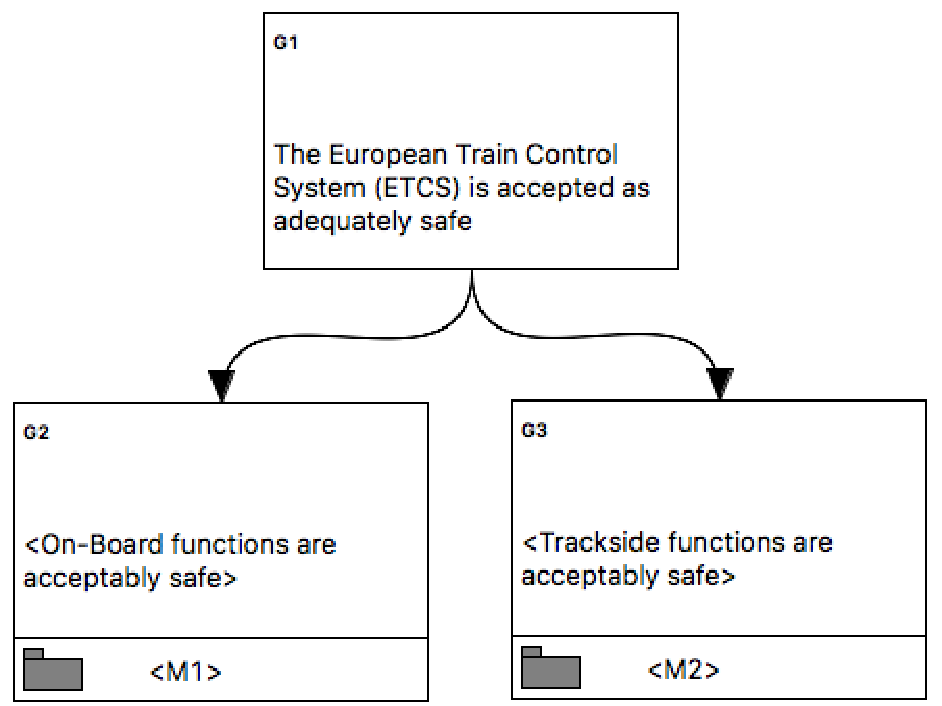
\includegraphics[width=\textwidth]{module_view.pdf}
		\caption{The Module View of ACME.}
		\label{fig:module_view}
	\end{minipage}
\end{figure}

ACME is implemented using the Graphical Modelling Framework (GMF) \cite{gmf}, which supports the creation of editors based on metamodels defined using the Ecore metamodel provided by the Eclipse Modelling Framework (EMF) \cite{steinberg2008emf}. 
As previously discussed, we created metamodels for GSN and CAE, the approach we take for ACME is to support GSN for the argumentation part of the assurance case (since there is no graphical syntax for the \textit{Argumentation} component of SACM).
In this sense, the users of ACME are able to create an assurance case using SACM, use GSN for the arguments, and then use SACM's \textit{Artifact} and \textit{Terminology} components for evidence-artefact traceability and controlled vocabulary. 
In this way, system assurance case practitioners are able to make the transition from GSN/CAE to SACM, from (mostly) non-model-based approach to uniformed model-based approach.

Figure~\ref{fig:ac_view} shows the Assurance Case Package View, within which the users are able to create Modules and Contract Modules of GSN, as well as elements defined in the \textit{AssuranceCase} component of SACM. 
Figure~\ref{fig:module_view} shows the Module view of ACME, where the users are able to create GSN elements. 

\begin{figure}
	\centering
	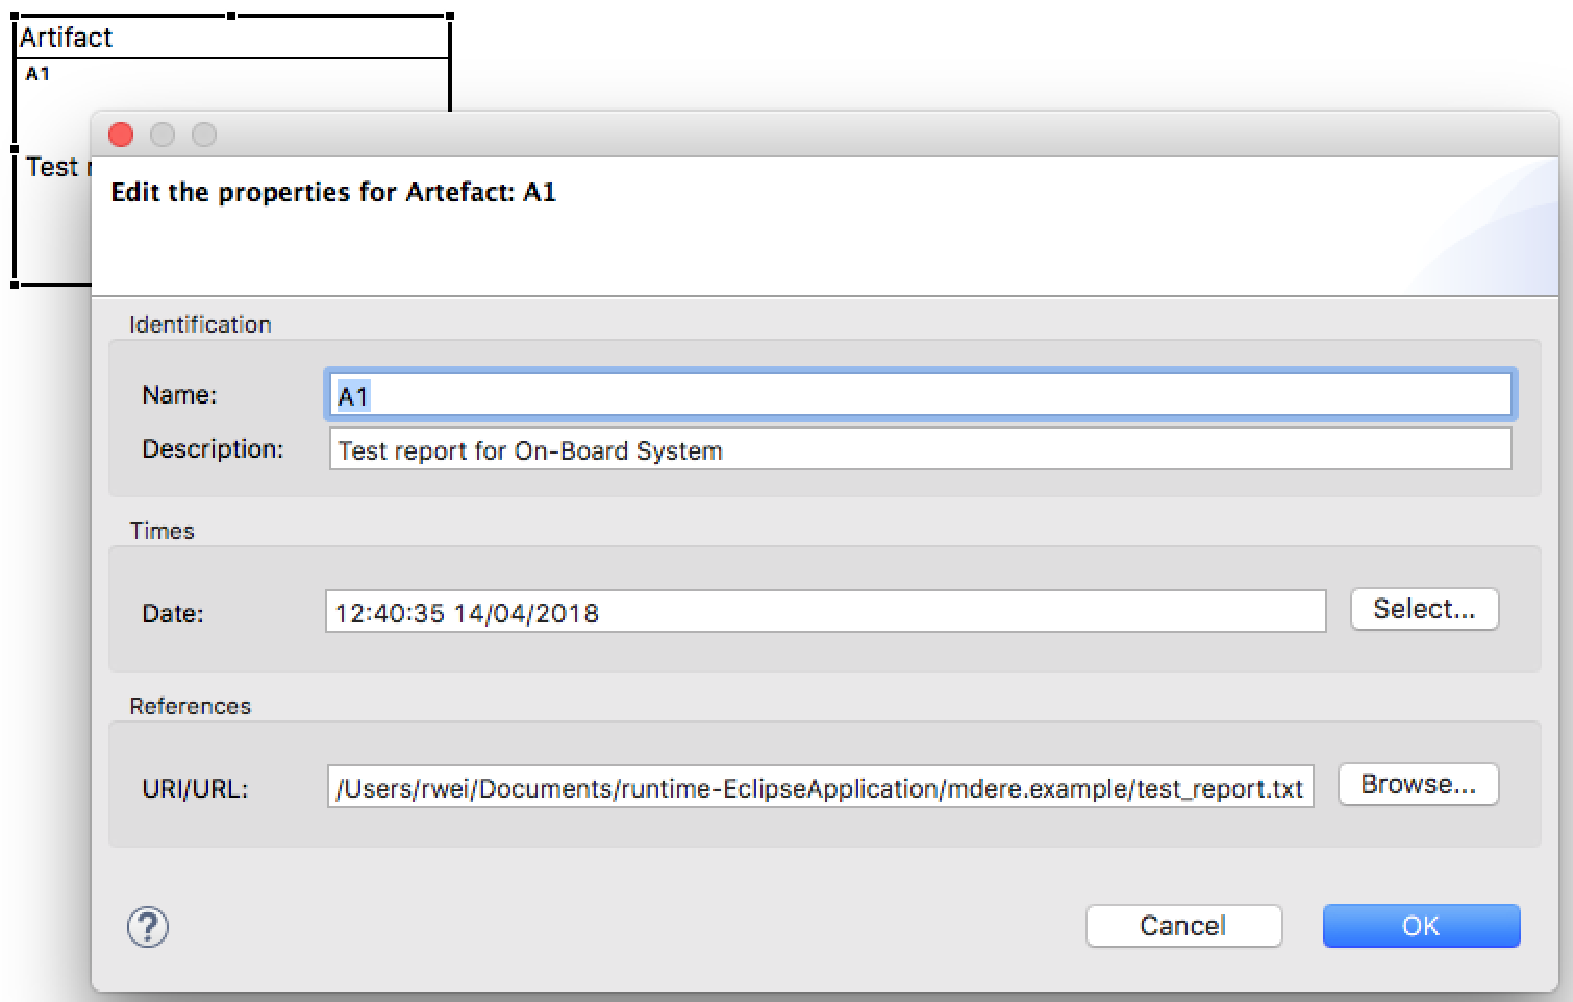
\includegraphics[width=.9\linewidth]{artifact_view.pdf}
	\caption{Creation of Artifact.}
	\label{fig:artifact_view}
\end{figure}

The users are also able to create elements in the \textit{Artifact} component of SACM (i.e. \textit{Artifact}, \textit{Activity}, \textit{Event}, \textit{Participant}, \textit{Technique}, \textit{Resource}, \textit{Property}, and \textit{ArtifactAssetRelationship}), Figure~\ref{fig:artifact_view} demonstrates how an \textit{Artifact} element can be created/edited. 
Creation tools are also provided for the elements in the \textit{Terminology} component, where a \textit{TerminologyPackage} is represented as a table in ACME, Figure~\ref{fig:terminology_view} demonstrates how a \textit{TerminologyPackage} and its contents can be created/edited.

\begin{figure}
	\centering
	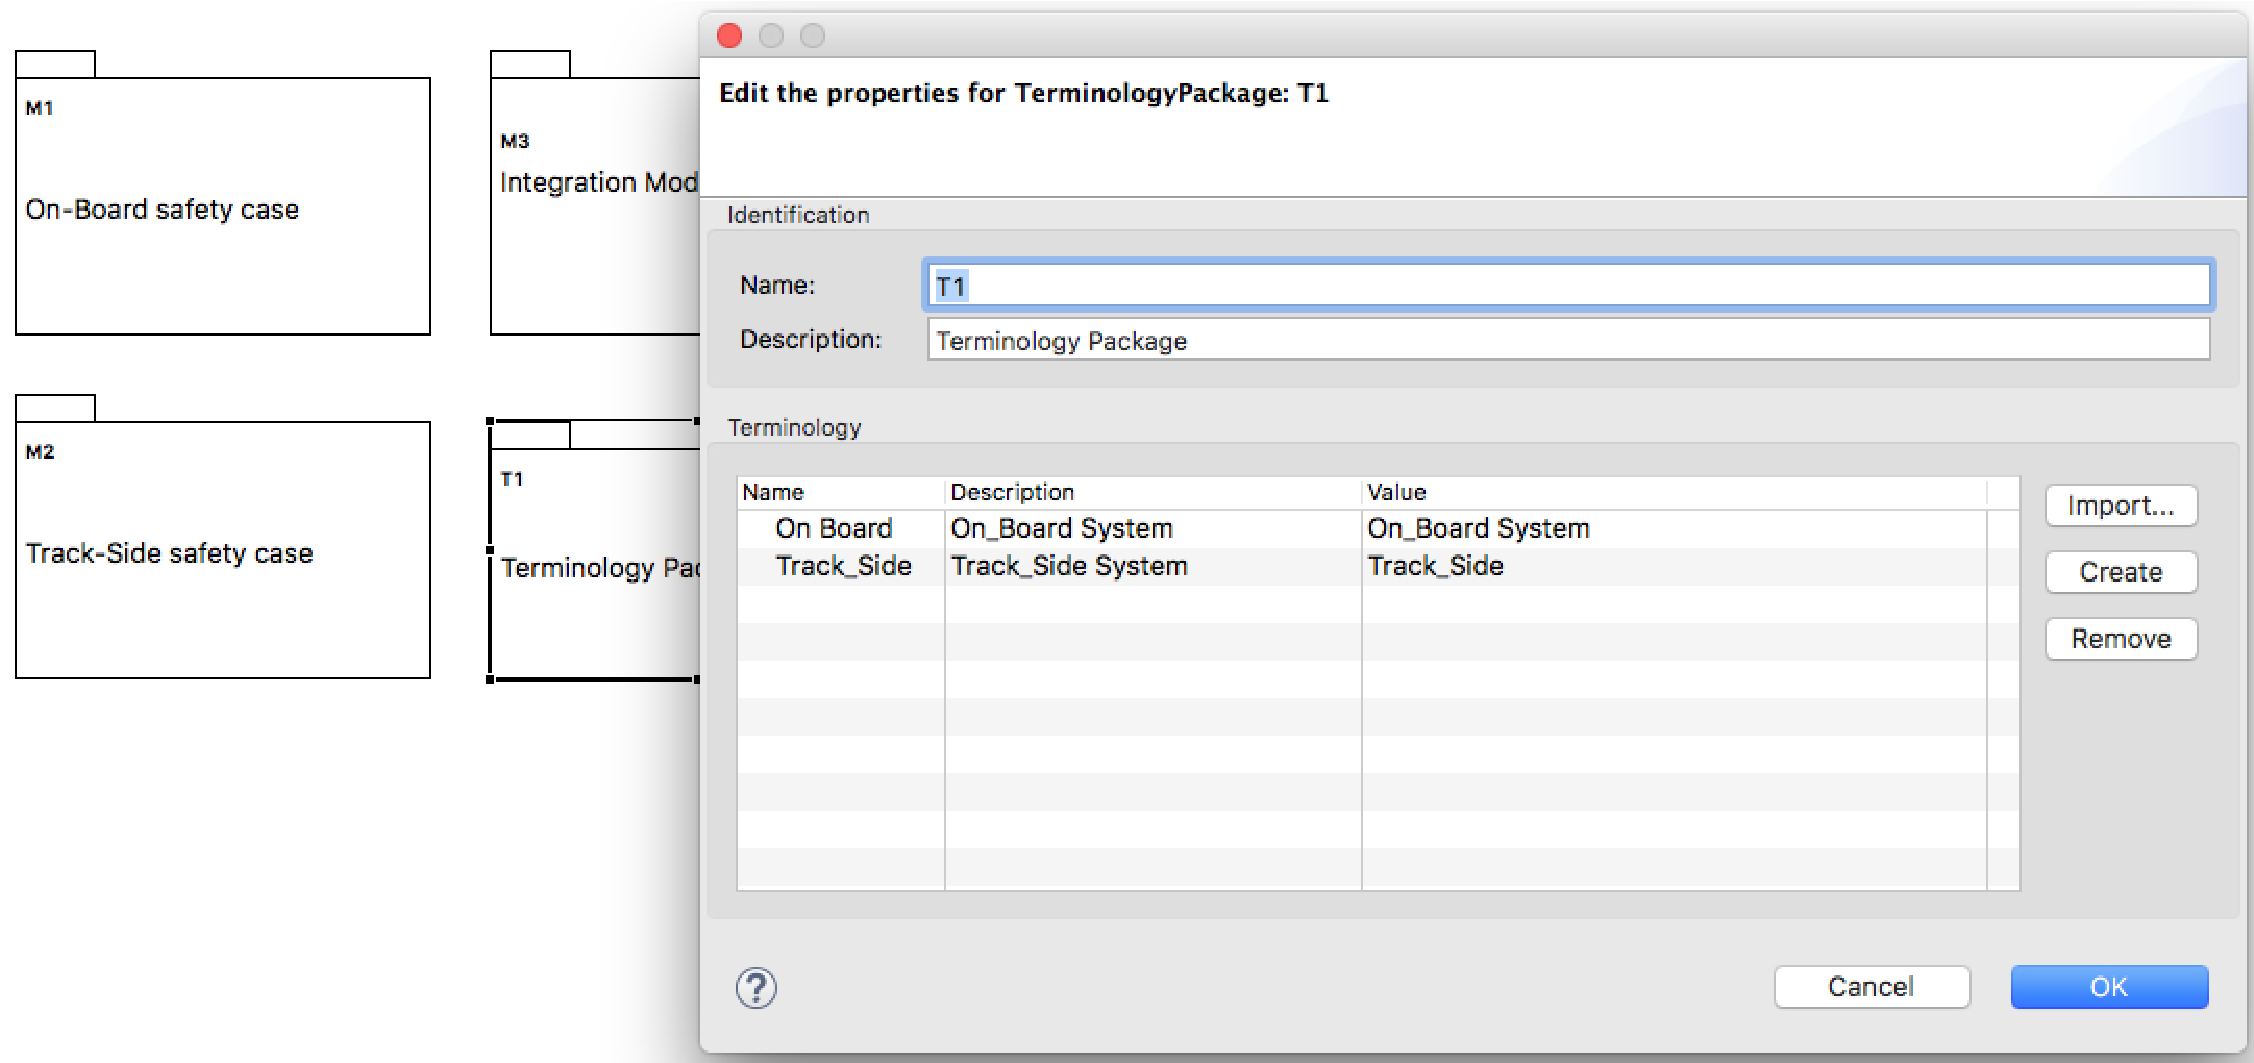
\includegraphics[width=1\linewidth]{terminology_view.pdf}
	\caption{Editing a \textit{TerminologyPackage}.}
	\label{fig:terminology_view}
\end{figure}

The idea behind ACME is to provide a transition for practitioners from GSN (and/or CAE\footnote{CAE editor for ACME is under development}) to SACM, before the OMG standardises the graphical syntax of SACM.
In this way, assurance case practitioners can continue use GSN, whilst exploiting the features provided by SACM (explained in Section~\ref{sec:ac_sacm}). 
\begin{figure}
	\centering
	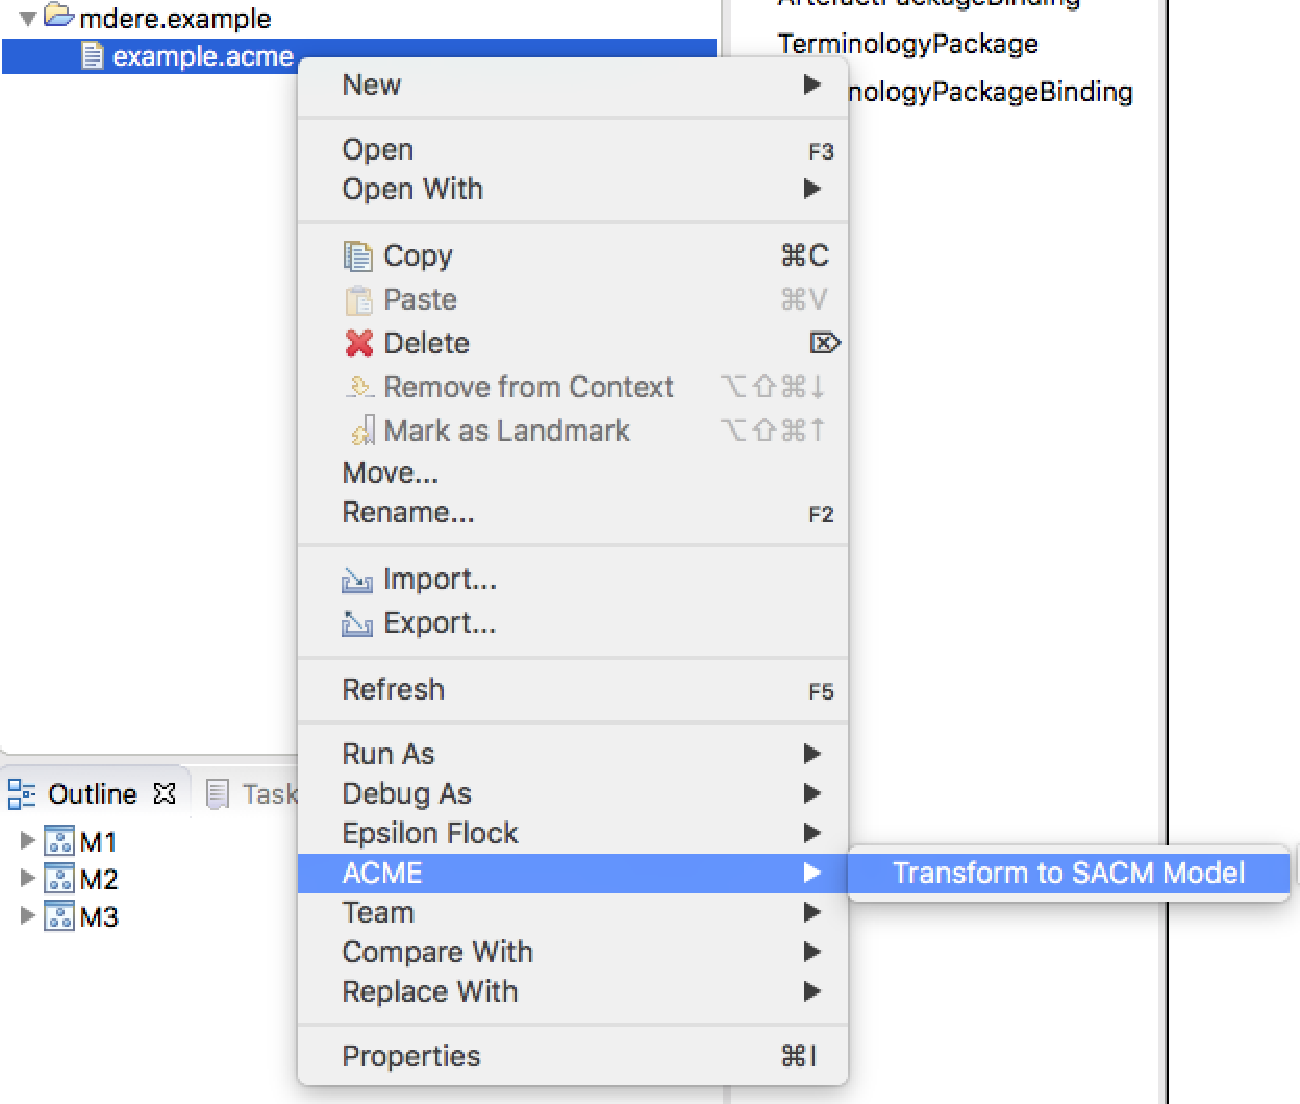
\includegraphics[width=.6\linewidth]{gsn2sacm_view.pdf}
	\caption{M2M function to transform a GSN model to a SACM model.}
	\label{fig:transformation_view}
\end{figure}

The users of ACME are also able to transform their GSN models to SACM, based on the model-to-model transformation from GSN to ACME. 
ACME integrates with the Epsilon platform, so that model management operations are supported on GSN/SACM models. 
A first step towards this direction is the support for GSN2SACM transformation, as shown in Figure~\ref{fig:transformation_view}.

ACME is the first step towards an integrated modelling environment for SACM.
ACME provides a transitional solution to model-based system assurance, in the sense that it enables existing assurance case approaches to be used in conjunction with SACM, in order to exploit the features provided by SACM such as evidence-artefact traceability, controlled vocabularies and multiple language support.
ACME as it is at the moment, illustrates what can be done with SACM and model-based assurance cases created with SACM.
However, it does not guarantee that assurance cases provided by ACME are compelling ones. 
It is still the responsibility of assurance case developers to develop accurate and correct assurance cases.

\subsection{Future Work}
With regard to future work for ACME, we aim at achieving the following;

\begin{itemize}
	\item Support for CAE. We aim to create the editor for CAE and integrate to ACME
	\item Support for legacy assurance cases. We aim to develop a set of model extraction mechanisms to extract information from assurance cases provided by existing tools and convert them to models that conform to our GSN/CAE metamodels.
	\item Model management programs. We aim to develop a set of model validation rules to check the well-formedness of GSN/CAE/SACM models. We also aim to develop a set of model-to-text transformation rules for assurance case report generation. Finally, 
	\item Support for automated pattern instantiation. We integrate the Epsilon platform runtime\footnote{\url{https://www.eclipse.org/epsilon/}} in ACME for various model management operations. We aim to explore how \textit{ImplementationConstraint}s can be utilised to hold Epsilon programs for pattern instantiation.
	\item Concrete syntax for SACM. We are contributing to the development of graphical notations for SACM at the moment, and will add the support for the notations in ACME once they are developed and evaluated.
\end{itemize}